\begin{figure}
    \centering
    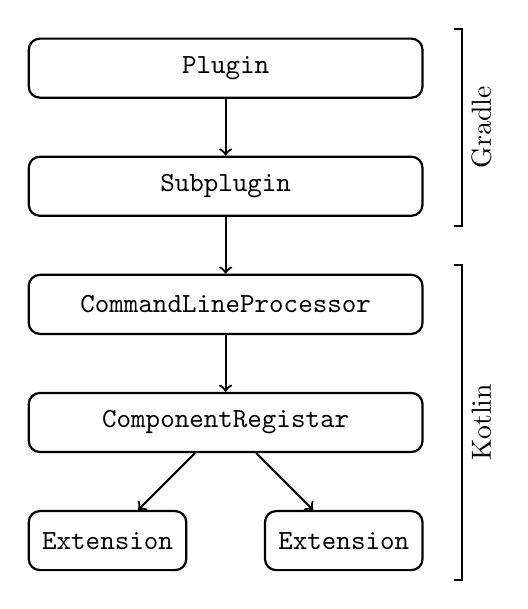
\begin{tikzpicture}
        \tikzstyle{layer}=[thick, rectangle, rounded corners, minimum height=7.5mm, minimum width=5cm, draw, font=\ttfamily]
        % \draw[draw=black!20] (-4,1) grid (4, -7);
        \node[layer] (plugin) at (0, 0) {Plugin};
        \node[layer] (subplugin) at (0, -1.5) {Subplugin};
        \node[layer] (cli-processor) at (0, -3) {CommandLineProcessor};
        \node[layer] (registar) at (0, -4.5) {ComponentRegistar};
        \node[layer, minimum width=2cm] (ext-left) at (-1.5, -6) {Extension};
        \node[layer, minimum width=2cm] (ext-right) at (1.5, -6) {Extension};

        \draw[->, thick] (plugin) -- (subplugin);
        \draw[->, thick] (subplugin) -- (cli-processor);
        \draw[->, thick] (cli-processor) -- (registar);
        \draw[->, thick] (registar) -- (ext-left);
        \draw[->, thick] (registar) -- (ext-right);

        \draw[thick] (2.9, 0.5) -- (3, 0.5) -- (3, -2) -- (2.9, -2);
        \draw[thick] (2.9, -2.5) -- (3, -2.5) -- (3, -6.5) -- (2.9, -6.5);

        \path (3, 0.5) -- node[below, rotate=90]{Gradle} (3, -2);
        \path (3, -2.5) -- node[below, rotate=90]{Kotlin} (3, -6.5);
    \end{tikzpicture}
    \caption{Kotlin compiler plugin architecture stack \autocite{Most2018}.}
    \label{fig:kotlin-compiler-plugin-arch}
\end{figure}